\section{main.cc File Reference}
\label{main_8cc}\index{main.cc@{main.cc}}
{\tt \#include $<$string$>$}\par
{\tt \#include $<$sstream$>$}\par
{\tt \#include $<$iostream$>$}\par
{\tt \#include $<$iomanip$>$}\par
{\tt \#include $<$cstdlib$>$}\par
{\tt \#include $<$fstream$>$}\par
{\tt \#include $<$map$>$}\par
{\tt \#include \char`\"{}../kernel/component.h\char`\"{}}\par
{\tt \#include \char`\"{}../kernel/simulator.h\char`\"{}}\par
{\tt \#include \char`\"{}../data\_\-types/impl/irisEvent.h\char`\"{}}\par
{\tt \#include \char`\"{}../MemCtrl/request.h\char`\"{}}\par
{\tt \#include \char`\"{}../MemCtrl/request\_\-handler.h\char`\"{}}\par
{\tt \#include \char`\"{}../MemCtrl/bus\_\-handler.h\char`\"{}}\par
{\tt \#include \char`\"{}../MemCtrl/bus.h\char`\"{}}\par
{\tt \#include \char`\"{}../MemCtrl/dram.h\char`\"{}}\par
{\tt \#include \char`\"{}../MemCtrl/NI.h\char`\"{}}\par
{\tt \#include \char`\"{}../MemCtrl/refresh\_\-manager.h\char`\"{}}\par
{\tt \#include \char`\"{}../MemCtrl/response\_\-handler.h\char`\"{}}\par
{\tt \#include \char`\"{}../MemCtrl/MC.h\char`\"{}}\par
{\tt \#include \char`\"{}../MemCtrl/mshr.h\char`\"{}}\par


Include dependency graph for main.cc:\nopagebreak
\begin{figure}[H]
\begin{center}
\leavevmode
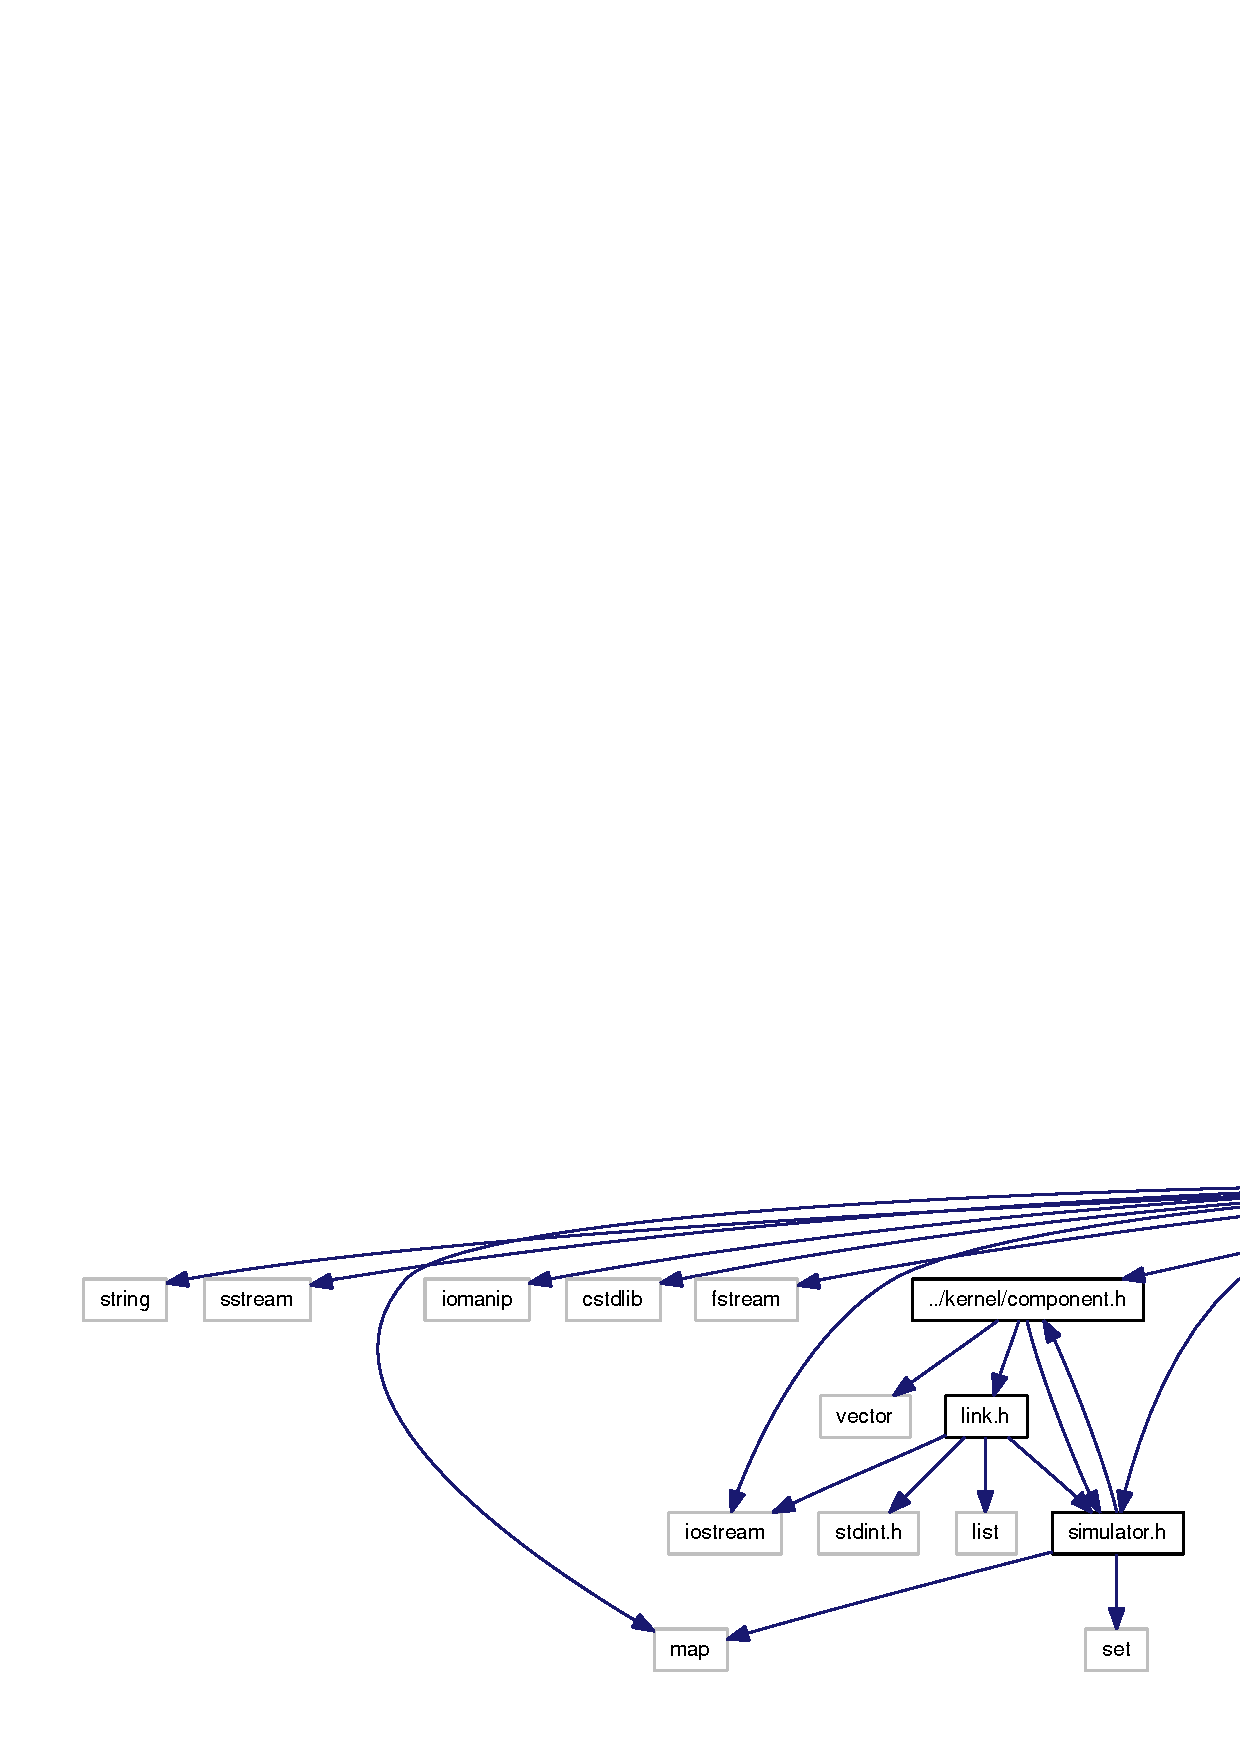
\includegraphics[width=420pt]{main_8cc__incl}
\end{center}
\end{figure}
\subsection*{Functions}
\begin{CompactItemize}
\item 
bool {\bf GetNextRequest} ({\bf MSHR\_\-H} {\bf mshrHandler}[$\,$], {\bf Request} $\ast$req, unsigned int $\ast$index)
\item 
int {\bf main} (int argc, char $\ast$$\ast$argv)
\end{CompactItemize}


\subsection{Function Documentation}
\index{main.cc@{main.cc}!GetNextRequest@{GetNextRequest}}
\index{GetNextRequest@{GetNextRequest}!main.cc@{main.cc}}
\subsubsection[{GetNextRequest}]{\setlength{\rightskip}{0pt plus 5cm}bool GetNextRequest ({\bf MSHR\_\-H} {\em mshrHandler}[$\,$], \/  {\bf Request} $\ast$ {\em req}, \/  unsigned int $\ast$ {\em index})}\label{main_8cc_3b0fd4edb104f5f9a3d5e25f3c554f06}




Definition at line 43 of file main.cc.

References MSHR\_\-H::lastScheduledIndex, MSHR\_\-H::mshr, NO\_\-OF\_\-THREADS, and MSHR\_\-H::writeQueue.\index{main.cc@{main.cc}!main@{main}}
\index{main@{main}!main.cc@{main.cc}}
\subsubsection[{main}]{\setlength{\rightskip}{0pt plus 5cm}int main (int {\em argc}, \/  char $\ast$$\ast$ {\em argv})}\label{main_8cc_3c04138a5bfe5d72780bb7e82a18e627}




Definition at line 100 of file main.cc.

References Request::address, Request::arrivalTime, Statistic::CalculateAggregateStats(), Request::cmdType, Statistic::CollectStatsPerCycle(), MSHR\_\-H::done, Statistic::doneOnce, IrisEvent::dst, IrisEvent::event\_\-data, MSHR\_\-H::filename, GetNextRequest(), MSHR\_\-H::GlobalAddrMap(), MSHR\_\-H::globalUnSink, Simulator::halted, MSHR\_\-H::id, mshrHandler, MC::ni, NO\_\-OF\_\-THREADS, Simulator::Now(), RequestHandler::oneBufferFull, Statistic::PrintAggregateStats(), RequestHandler::process\_\-event(), MSHR\_\-H::process\_\-event(), MC::reqH, Simulator::Run(), Simulator::Schedule(), IrisEvent::src, START, MC::stats, Simulator::StopAt(), Request::threadId, MSHR\_\-H::trace\_\-filename, IrisEvent::type, and MSHR\_\-H::unsink.